\documentclass[twoside,a4paper]{article}

\usepackage{amsmath}
\usepackage{amssymb}
\usepackage[left=1in,right=1in,top=1in,bottom=1in]{geometry}
\usepackage{enumitem}
\usepackage{parskip}
\usepackage{booktabs}
\usepackage{graphicx}
\usepackage[hidelinks]{hyperref}
\usepackage{caption}
\usepackage{subcaption}
\usepackage{longtable}
\usepackage{biblatex}
\usepackage{xspace}
\usepackage{tikz-feynhand}

\addbibresource{bibliography.bib}

\setlist[itemize]{label=$\cdot$,leftmargin=1em}
\setlength{\parskip}{1em}

% Custom commands
\newcommand{\ttH}{\ensuremath{{t\bar{t}H}}\xspace}
\newcommand{\tth}{\ttH}

\title{Further optimization of the \ttH signal and background separation using deep learning in the
    $2l_{SS}1\tau$ channel.}

\author{Vladyslav Yazykov}
\date{}

% Glossaries
\usepackage{glossaries}

\newacronym{sr}{SR}{Signal Region}
\newacronym{dsid}{DSID}{Dataset ID}


% Change the \includeonly later
\includeonly{sections/mu/_section.tex}

\begin{document}

% Title
\maketitle

% Glossaries
\printglossary[type=\acronymtype,title=Abbreviations]

% Main sections
\section{Introduction}

In this study we aim to further improve the performance of the classifier used to separate the process of interest
($t\bar{t}H$) from the background processes.

We have moved to the version 8 of the ntuples, and have also made changes to the optimization part itself. We have applied the
transformer architecture, experimented with fine-tuning, tried different weight configurations, and have experimented
with the training on the extended dataset, obtained by dropping all the selection cuts. We have experimented with
different feature sets, and have proposed an automated way of selecting the well-modelled features.

We have evaluated the uncertainty on the median signal strength parameter $\mu_{t\bar{t}H}$, considering both the
statistical and systematical uncertainties.
\section{V8 adaptation}

\subsection{\gls{sr} details}

{\scriptsize
    \begin{verbatim}
    custTrigMatch_LooseID_FCLooseIso_DLT
    && (dilep_type && (lep_ID_0*lep_ID_1)>0)
    && ((lep_Pt_0 >= 10e3 && lep_Pt_1 >= 10e3) && (fabs(lep_Eta_0) <= 2.5 && fabs(lep_Eta_1) <= 2.5)
        && ((abs(lep_ID_0) == 13 && lep_isMedium_0 && lep_isolationLoose_VarRad_0 && passPLIVTight_0)
            || ((abs(lep_ID_0) == 11 && lep_isTightLH_0 && lep_isolationLoose_VarRad_0 && passPLIVTight_0
                && lep_ambiguityType_0 == 0 && lep_chargeIDBDTResult_recalc_rel207_tight_0 > 0.7)
                && ((!(!(lep_Mtrktrk_atConvV_CO_0 < 0.1 && lep_Mtrktrk_atConvV_CO_0 >= 0 && lep_RadiusCO_0 > 20)
                    && (lep_Mtrktrk_atPV_CO_0 < 0.1 && lep_Mtrktrk_atPV_CO_0 >= 0)))
                    && !(lep_Mtrktrk_atConvV_CO_0 <0.1 && lep_Mtrktrk_atConvV_CO_0 >= 0 && lep_RadiusCO_0 > 20))))
            && ((abs(lep_ID_1) == 13 && lep_isMedium_1 && lep_isolationLoose_VarRad_1 && passPLIVTight_1)
                || ((abs(lep_ID_1) == 11 && lep_isTightLH_1 && lep_isolationLoose_VarRad_1 && passPLIVTight_1
                    && lep_ambiguityType_1 == 0 && lep_chargeIDBDTResult_recalc_rel207_tight_1 > 0.7)
                    && ((!(!(lep_Mtrktrk_atConvV_CO_1 < 0.1 && lep_Mtrktrk_atConvV_CO_1 >= 0 && lep_RadiusCO_1 > 20)
                        && (lep_Mtrktrk_atPV_CO_1 < 0.1 && lep_Mtrktrk_atPV_CO_1 >= 0)))
                        && !(lep_Mtrktrk_atConvV_CO_1 < 0.1 && lep_Mtrktrk_atConvV_CO_1 >= 0 && lep_RadiusCO_1 > 20)))))
    && nTaus_OR==1
    && nJets_OR_DL1r_85>=1
    && nJets_OR>=4
    && ((dilep_type==2) || abs(Mll01-91.2e3)>10e3)
\end{verbatim}
}

We have kept the cuts essentially the same, except for the cut on the \verb|nJets_OR| to \verb|>=4| to keep consistent
\gls{sr} definition across the group.

\subsection{List of samples by each process}

The root directory for the files is:

{\small
\verb|/eos/atlas/atlascerngroupdisk/phys-higgs/HSG8/multilepton_ttWttH/v08/v0801/systematics-full/nominal|
}

The list of samples is given in \hyperref[tab:samples]{Table~\ref*{tab:samples}}.

\newpage

\begin{table}[h!]
    \centering
    \renewcommand{\arraystretch}{1.5}
    \caption{List of samples by each process}
    \label{tab:samples}
    \begin{tabular}{p{1.5cm}p{13.5cm}}
        \toprule
        Process      & \gls{dsid}                                                           \\
        \midrule
        $t\bar{t}H$  & p4498/346343, p4498/346344, p4498/346345                             \\
        $t\bar{t}W$  & p4416/700168, p4590/700205                                           \\
        $t\bar{t}Z$  & p4416/700168                                                         \\
        $t\bar{t}$   & p4308/410470                                                         \\
        $VV$         & p4416/364250, p4416/364253, p4416/364254, p4416/364255, p4308/364283, p4308/364284, p4308/364285,
p4308/364286, p4308/364287, p4308/363355, p4308/363356, p4308/363357, p4308/363358, p4308/363359,
p4308/363360, p4308/363489                                               \\
        $ggVV$       & p4308/345705, p4396/345706, p4396/345715, p4396/345718, p4396/345723 \\
        $Zjets$      & p4308/364100, p4308/364101, p4308/364102, p4308/364103, p4308/364104, p4308/364105, p4308/364106,
p4308/364107, p4308/364108, p4308/364109, p4308/364110, p4308/364111, p4308/364112, p4308/364113,
p4308/364114, p4308/364115, p4308/364116, p4308/364117, p4308/364118, p4308/364119, p4308/364120,
p4308/364121, p4308/364122, p4308/364123, p4308/364124, p4308/364125, p4308/364126, p4308/364127,
p4308/364128, p4308/364129, p4308/364130, p4308/364131, p4308/364132, p4308/364133, p4308/364134,
p4308/364135, p4308/364136, p4308/364137, p4308/364138, p4308/364139, p4308/364140, p4308/364141,
p4308/364198, p4308/364199, p4308/364200, p4308/364201, p4308/364202, p4308/364203, p4308/364204,
p4308/364205, p4308/364206, p4308/364207, p4308/364208, p4308/364209, p4308/364210, p4308/364211,
p4308/364212, p4308/364213, p4308/364214, p4308/364215                                            \\
        $Wjets$      & p4308/364156, p4308/364157, p4308/364158, p4308/364159, p4308/364160, p4308/364161, p4308/364162,
p4308/364163, p4308/364164, p4308/364165, p4308/364166, p4308/364167, p4308/364168, p4308/364169,
p4308/364170, p4308/364171, p4308/364172, p4308/364173, p4308/364174, p4308/364175, p4308/364176,
p4308/364177, p4308/364178, p4308/364179, p4308/364180, p4308/364181, p4308/364182, p4308/364183,
p4308/364184, p4308/364185, p4308/364186, p4308/364187, p4308/364188, p4308/364189, p4308/364190,
p4308/364191, p4308/364192, p4308/364193, p4308/364194, p4308/364195, p4308/364196, p4308/364197                                            \\
        $tW$         & p4308/410646, p4308/410647                                           \\
        $threeTop$   & p4308/304014                                                         \\
        $fourTop$    & p4308/410080                                                         \\
        $t\bar{t}WW$ & p4308/410081                                                         \\
        $tZ$         & p4308/410560                                                         \\
        $WtZ$        & p4308/410408                                                         \\
        $VVV$        & p4308/364242, p4308/364243, p4308/364244, p4308/364245, p4308/364246, p4308/364247, p4308/364248, p4308/364249                                              \\
        $VH$         & p4308/342284, p4308/342285                                           \\
        $tHjb$       & p4308/346799\_AF                                                     \\
        $tWH$        & p4308/346678\_AF                                                     \\
        \bottomrule
    \end{tabular}
\end{table}

\newpage
\subsection{Distribution of the variables inside \gls{sr}}

The following figures (\autoref{fig:distributions1} and \autoref{fig:distributions2}) show the distributions of some variables
of interest inside \gls{sr}.

\captionsetup[subfigure]{justification=centering}
\begin{figure}[htb!]
    \centering
    \begin{subfigure}{0.45\textwidth}
        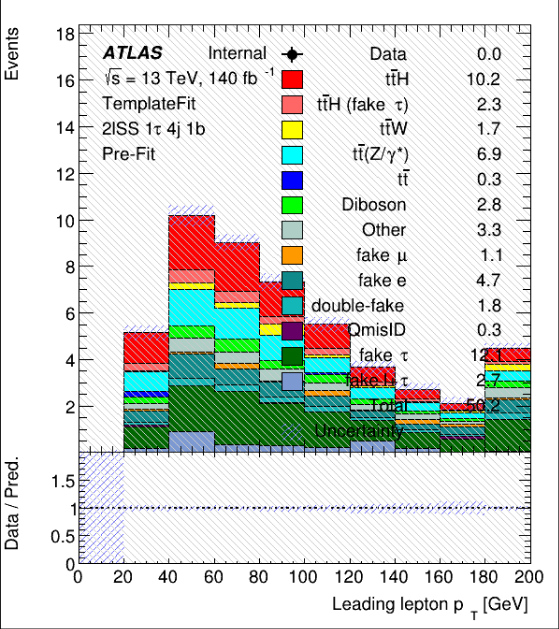
\includegraphics[width=\linewidth]{figures/plots/histograms/lep_pt_0.png}
        \caption{Distribution of the transverse momentum of the leading lepton.}
        \label{fig:lep_pt_0}
    \end{subfigure}\hfill%
    \begin{subfigure}{0.45\textwidth}
        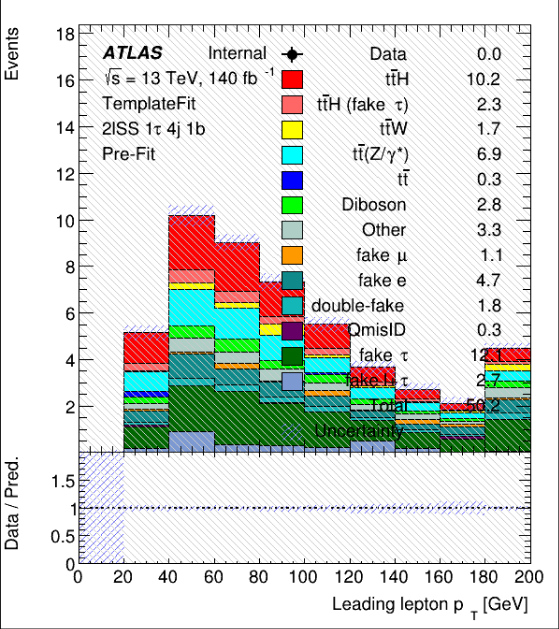
\includegraphics[width=\linewidth]{figures/plots/histograms/lep_pt_1.png}
        \caption{Distribution of the transverse momentum of the subleading lepton.}
        \label{fig:lep_pt_1}
    \end{subfigure}

    \vspace{0.5cm}

    \begin{subfigure}{0.45\textwidth}
        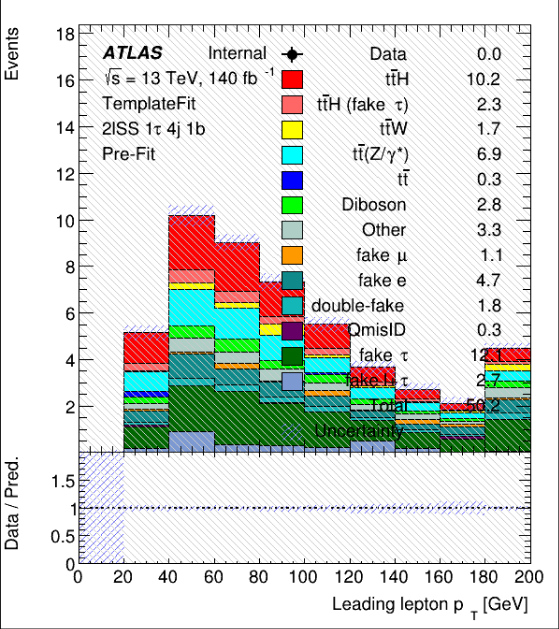
\includegraphics[width=\linewidth]{figures/plots/histograms/lep_Eta_0.png}
        \caption{Distribution of the pseudorapidity of the leading lepton.}
        \label{fig:lep_Eta_0}
    \end{subfigure}\hfill%
    \begin{subfigure}{0.45\textwidth}
        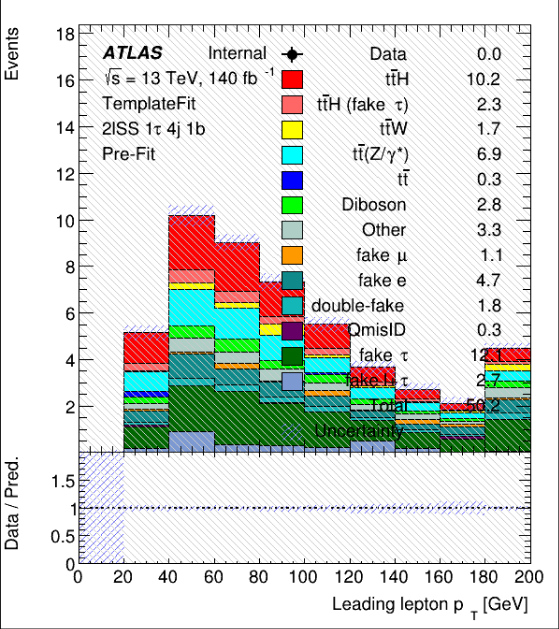
\includegraphics[width=\linewidth]{figures/plots/histograms/lep_Eta_1.png}
        \caption{Distribution of the pseudorapidity of the subleading lepton.}
        \label{fig:lep_Eta_1}
    \end{subfigure}
    \caption{Distributions of the variables inside \gls{sr} (part 1)}
    \label{fig:distributions1}
\end{figure}

\newpage

\begin{figure}[htb!]
    \centering
    \begin{subfigure}{0.45\textwidth}
        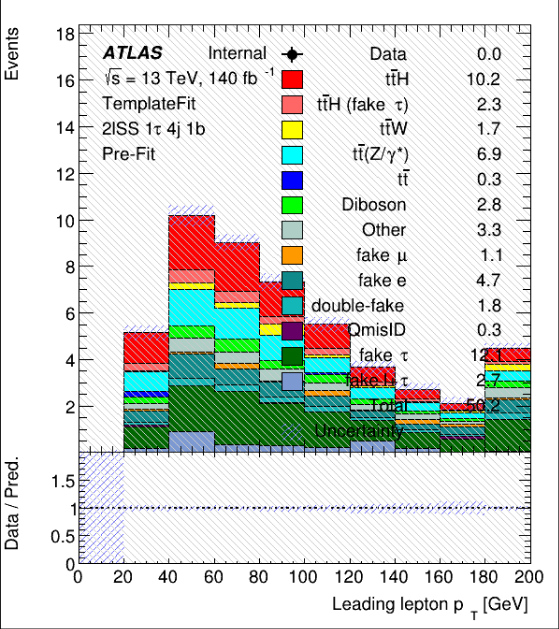
\includegraphics[width=\linewidth]{figures/plots/histograms/lep_Phi_0.png}
        \caption{Distribution of the azimuthal angle of the leading lepton.}
        \label{fig:lep_Phi_0}
    \end{subfigure}\hfill%
    \begin{subfigure}{0.45\textwidth}
        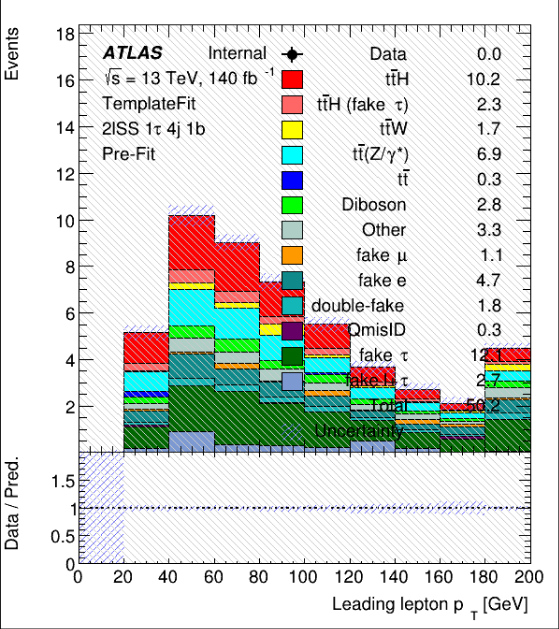
\includegraphics[width=\linewidth]{figures/plots/histograms/lep_Phi_1.png}
        \caption{Distribution of the azimuthal angle of the subleading lepton.}
        \label{fig:lep_Phi_1}
    \end{subfigure}

    \vspace{0.5cm}

    \begin{subfigure}{0.45\textwidth}
        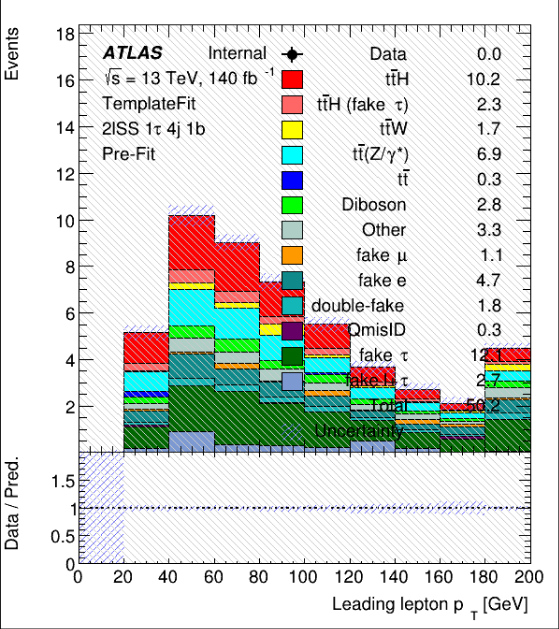
\includegraphics[width=\linewidth]{figures/plots/histograms/njets.png}
        \caption{Distribution of the number of jets.}
        \label{fig:njets}
    \end{subfigure}\hfill%
    \begin{subfigure}{0.45\textwidth}
        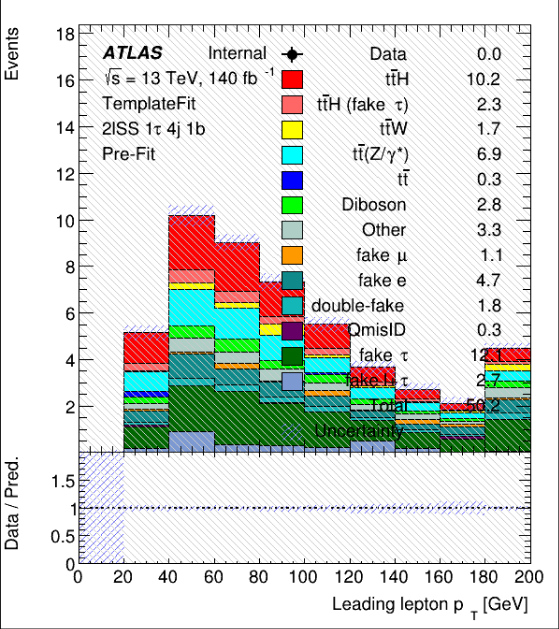
\includegraphics[width=\linewidth]{figures/plots/histograms/nbjets.png}
        \caption{Distribution of the number of $b$-jets.}
        \label{fig:nbjets}
    \end{subfigure}
    \caption{Distributions of the variables inside \gls{sr} (part 2)}
    \label{fig:distributions2}
\end{figure}

\begin{minipage}{0.45\textwidth}
    \centering
    \begin{tabular}{c|c|c|c|c}
        $t\bar{t}H$ & \textbf{v6} & \textbf{v8} &      &       \\
        \hline
        Weighted    & 1000        & 500         & -500 & -50\% \\
        Raw         & 1000        & 500         & -500 & -50\% \\
        \hline
    \end{tabular}
    \captionof{table}{Number of ttH events in the SR for v6 and v8.}
    \label{tab:ttH_event_numbers1}
\end{minipage}\hfill%
\begin{minipage}{0.45\textwidth}
    \centering
    \begin{tabular}{c|c|c|c|c}
        \gls{sr} & \textbf{v6} & \textbf{v8} &      &       \\
        \hline
        Weighted & 1000        & 500         & -500 & -50\% \\
        Raw      & 1000        & 500         & -500 & -50\% \\
        \hline
    \end{tabular}
    \captionof{table}{Number of all the events in the SR for v6 and v8.}
    \label{tab:ttH_event_numbers2}
\end{minipage}

\subsection{New/changed features}

This can just be a table with:

\begin{longtable}{ll}
    \hline
    \textbf{Feature}             & \textbf{Importance}          \\ \hline
    \endfirsthead

    \multicolumn{2}{c}%
    {{\bfseries Table \thetable\ continued from previous page}} \\
    \hline
    \textbf{Feature}             & \textbf{Importance}          \\ \hline
    \endhead

    \hline \multicolumn{2}{|r|}{{Continued on next page}}       \\ \hline
    \endfoot

    \hline
    \endlastfoot

    HT                           & 1.2                          \\
    HT\_fwdJets                  & 2.5                          \\
    HT\_inclFwdJets              & 1.8                          \\
    HT\_lep                      & 3.1                          \\
    HT\_jets                     & 2.7                          \\
    HT\_taus                     & 2.9                          \\
    jets\_eta\_0                 & 5.0                          \\
    jets\_pt\_0                  & 4.8                          \\
    jets\_e\_0                   & 4.9                          \\
    jets\_phi\_0                 & 4.7                          \\
    jets\_eta\_1                 & 2.3                          \\
    jets\_pt\_1                  & 2.1                          \\
    jets\_e\_1                   & 2.2                          \\
    jets\_phi\_1                 & 2.0                          \\
    jets\_eta\_2                 & 1.5                          \\
    jets\_pt\_2                  & 1.3                          \\
    jets\_e\_2                   & 1.4                          \\
    jets\_phi\_2                 & 1.2                          \\
    jets\_eta\_3                 & 0.9                          \\
    jets\_pt\_3                  & 0.8                          \\ \hline
    jets\_e\_3                   & 0.8                          \\
    jets\_phi\_3                 & 0.7                          \\
    jets\_eta\_4                 & 0.5                          \\
    jets\_pt\_4                  & 0.4                          \\
    jets\_e\_4                   & 0.4                          \\
    jets\_phi\_4                 & 0.3                          \\
    jets\_eta\_5                 & 0.2                          \\
    jets\_pt\_5                  & 0.1                          \\
    jets\_e\_5                   & 0.1                          \\
    jets\_phi\_5                 & 0.1                          \\
    lep\_E\_0                    & 3.5                          \\
    lep\_E\_1                    & 3.4                          \\
    lep\_Eta\_0                  & 1.6                          \\
    lep\_Eta\_1                  & 1.5                          \\
    lep\_EtaBE2\_0               & 1.2                          \\
    lep\_EtaBE2\_1               & 1.1                          \\
    lep\_ID\_0                   & 1.8                          \\
    lep\_ID\_1                   & 1.7                          \\
    lep\_ambiguityType\_0        & 1.1                          \\
    lep\_ambiguityType\_1        & 1.0                          \\
    lep\_sigd0PV\_0              & 2.3                          \\
    lep\_sigd0PV\_1              & 2.2                          \\
    Mb1                          & 1.3                          \\
    lep\_Mtrktrk\_atConvV\_CO\_0 & 1.5                          \\
    lep\_Mtrktrk\_atConvV\_CO\_1 & 1.4                          \\
    lep\_Mtrktrk\_atPV\_CO\_0    & 1.3                          \\
    lep\_Mtrktrk\_atPV\_CO\_1    & 1.2                          \\
    lep\_nInnerPix\_0            & 1.0                          \\
    lep\_nInnerPix\_1            & 0.9                          \\
    lep\_nTrackParticles\_0      & 1.1                          \\
    lep\_nTrackParticles\_1      & 1.0                          \\
    lep\_Phi\_0                  & 1.6                          \\
    lep\_Phi\_1                  & 1.5                          \\
    lep\_Pt\_0                   & 2.1                          \\
    lep\_Pt\_1                   & 2.0                          \\
    lep\_sigd0PV\_0              & 2.3                          \\
    lep\_sigd0PV\_1              & 2.2                          \\
    lep\_Z0SinTheta\_0           & 1.3                          \\
    lep\_Z0SinTheta\_1           & 1.2                          \\
    max\_eta                     & 1.4                          \\
    met\_met                     & 2.6                          \\
    met\_phi                     & 2.5                          \\
    taus\_DL1r\_0                & 2.4                          \\
    taus\_charge\_0              & 1.9                          \\
    taus\_decayMode\_0           & 1.8                          \\
    taus\_eta\_0                 & 2.0                          \\
    taus\_fromPV\_0              & 1.7                          \\
    taus\_numTrack\_0            & 1.6                          \\
    taus\_passEleBDT\_0          & 1.5                          \\
    taus\_passEleOLR\_0          & 1.4                          \\
    taus\_passJVT\_0             & 1.3                          \\
    taus\_phi\_0                 & 2.1                          \\
    taus\_pt\_0                  & 2.0                          \\
    taus\_width\_0               & 1.9                          \\
    minDeltaR\_LJ\_0             & 1.1                          \\
    minDeltaR\_LJ\_1             & 1.0                          \\
    minDeltaR\_LJ\_2             & 0.9                          \\
    minOSMll                     & 1.2                          \\
    minOSSFMll                   & 1.1                          \\
    mjjMax\_frwdJet              & 1.7                          \\
    MLepMet                      & 2.3                          \\
    Mll01                        & 2.2                          \\
    Mlll012                      & 2.1                          \\
    Mllll0123                    & 2.0                          \\
    MtLepMet                     & 2.6                          \\
    nFwdJets\_OR                 & 1.8                          \\
    nJets\_OR                    & 2.4                          \\
    nTaus\_OR\_Pt25              & 2.3                          \\
    Ptll01                       & 2.2                          \\
    sumPsbtag                    & 1.9                          \\
    total\_charge                & 1.6                          \\
    Mlb                          & 1.7                          \\
    total\_leptons               & 1.5                          \\
    passPLIVTight\_0             & 2.0                          \\
    passPLIVTight\_1             & 1.9                          \\
    nJets\_OR\_DL1r\_77          & 1.4                          \\
    nTaus\_OR                    & 1.3                          \\
    best\_Z\_Mll                 & 1.6                          \\
    best\_Z\_other\_Mll          & 1.5                          \\
    best\_Z\_other\_MtLepMet     & 1.4                          \\
    DeltaR\_min\_lep\_jet        & 2.0                          \\
    DeltaR\_min\_lep\_jet\_fwd   & 1.9                          \\
    dEta\_maxMjj\_frwdjet        & 1.8                          \\
    dilep\_type                  & 1.7                          \\
    DRll01                       & 2.2                          \\
    DeltaR\_max\_lep\_bjet77     & 2.1                          \\
    DRjj\_lead                   & 2.0                          \\
    eta\_frwdjet                 & 1.9                          \\
    flag\_JetCleaning\_LooseBad  & 1.8                          \\
    MtLep1Met                    & 2.4                          \\
    \caption{Feature Importance}
    \label{tab:feature_importance}
\end{longtable}



\section{Optimization improvements}


\subsection{Baseline - mlp/resnet}

\begin{itemize}
    \item Severin just used MLPs. He also tried combining the MLPs together, but this is fundamentally the same stuff -
          just a big MLP.
    \item As a baseline, we use a slightly improved version of it - with residual connections. We refer to it as ResNet.
    \item Describe that better to use deep nets then wide, because wide ResNets can juts memorize and overfit easily.
\end{itemize}


\subsection{Feature Tokenizer - Transformer (FT-Transformer)}

(Refer to the same paper.)


\subsection{Increasing statistics by dropping the cuts}

\begin{enumerate}
    \item Does it make much difference for transformers and ResNets both or only for transformers?
    \item How do BDT behave in this case?
\end{enumerate}

\subsection{Trying to differentiate between all the classes, or just signal and background?}

Severin has done this experiment as well, but we take it one step further. First, we evaluate how do the models perform
when we try to differentiate between all the classes, compared to just signal and background.

Then, we compare it with training on all the classes, and fine-tuning on signal and background only.


\subsection{Using (or not using?) event weights \em{correctly}}

\textbf{The meaning of Cross-Entropy loss weights is very different from the standard event weights.}

E.g. how should the event weights be used. Explain that Severin has not used them correctly,
but we don't really know how to use them correctly.

(We should present the training runs with and without weights. For different configurations.)

Maybe just write that we didn't use the weights during the training, so we don't need to re-weight anything.


\subsection{Effect of the reduced training set size}

Interestingly, we observe some strange stuff.

From $10\% \rightarrow 20\% \rightarrow 50\% \rightarrow 80\%$ performance increases have diminishing returns.
But from $80\% \rightarrow 100\%$ the performance increase is much larger.

I also don't understand why \verb|trn/loss| is different for different training set sizes. As we should just use the
average.

Also, I cannot reproduce my initial results with very high AUC scores. I don't know what I did wrong. But looks like I
messed up with the features somewhere along the way. Or maybe it's indeed the scale factors (SF)?


\subsection{Effect of the reduced feature set}

Reducing the total number of features reduces the systematical uncertainties. That is why it's best to have as few
features as possible. However, the trade-off is that we lose some information which likely leads to a reduced
performance of the classifier.

Furthermore, to have trustworthy results, we need to make sure the features used are well modelled. That is, the
distributions of the features in the simulated data agrees with the recorded data well enough.

Selected feature sets:

\begin{itemize}
    \item All features
    \item Only well-modelled features
    \item Top 20 most important features (from all features)
    \item Top 20 best modelled features
    \item Top 20 most important (of the well-modelled)
    \item Top 20 features with least systematical uncertainty contribution (is this possible?)
    \item Nello's features
\end{itemize}



\subsection{Results, comparison between different models}

\begin{itemize}
    \item ROCs + AUCs
    \item Significance, threshold scanning, thresholds
    \item Confusion matrices (for different thresholds)
    \item NN output - ttH probability distribution
\end{itemize}

\section{$\mu_{t\bar{t}H}$ - median signal strength estimation}

Uncertainty using just the statistical uncertainty is:

$$
    \mu_{t\bar{t}H} + 0.999 /-0.999
$$

By including the systematical uncertainty, we get:

$$
    \mu_{t\bar{t}H} + 0.999 /-0.999
$$


\section{Conclusions}

We have made a very important research.

\section{Appendix}


\subsection{Automated well-modelling estimation}

This "well enough" usually just means that a person looks at the plots and decides if the agreement is good enough.
But we propose an automated way of doing this. As the algorithm is basically checking if the number of weighted events
in each bin is the same for the simulated and recorded data. However, only the bins where the signal to background ratio
is high enough are considered.

Each bin thus contributes to the well-modelling score. If the bin is blinded, the contribution is zero. Otherwise, the
contribution for the bin is:

$$
    \text{Bin Contribution} = 1 - \frac{N_\text{Recorded} - N_\text{Simulation}}{\max(N_\text{Recorded}, N_\text{Simulation})}
$$

Where $N_\text{Recorded}$ and $N_\text{Simulation}$ are the number of weighted events in the bin for the recorded and
simulated data respectively.

The total well-modelling score is then the mean of the contributions for all the bins.



\subsection{Training times}

Training transformers takes long and has a large carbon footprint.

% Feynman diagram example
% \begin{equation}
%     \begin{tikzpicture}
%         \begin{feynhand}
%             \vertex[ringdot,label=above:{s}] (v) at (0,0) {};
%             \vertex[right=of v] (f1) ;
%             \vertex [above left=of v] (i1);
%             \vertex [below left=of v] (i2);
%             \propag [fermion, momentum'=\(p_1\)] (i1) to (v);
%             \propag [anti fermion,momentum'=\(p_2\)] (i2) to (v);
%             \propag [boson, momentum'=\(p_3\)] (v) to (f1);
%         \end{feynhand}
%     \end{tikzpicture}
% \end{equation}

% Bibliography
\printbibliography

\end{document}